Este capítulo apresentará o método proposto por este trabalho para o projeto de uma prótese ativa baseada em sensores e aprendizado de máquina.

\section{Visão geral do método}\label{sec:metodo_protese}

O projeto desenvolvido neste trabalho é uma prótese robótica para membros inferiores ou, mais especificamente, para a articulação do tornozelo. Esta prótese será construída a partir de modelos de próteses para impressoras 3D, aproveitando-se as partes mecânicas. A intenção é manter um baixo custo de produção. O sistema é projetado para funcionar em uma prótese transtibial, atuando sobre ela para adaptar a rigidez da articulação conforme a situação.

\begin{figure}[h]
	\caption{\label{fig:big_picture}Visão geral do protótipo}
	\begin{center}
	    \fbox{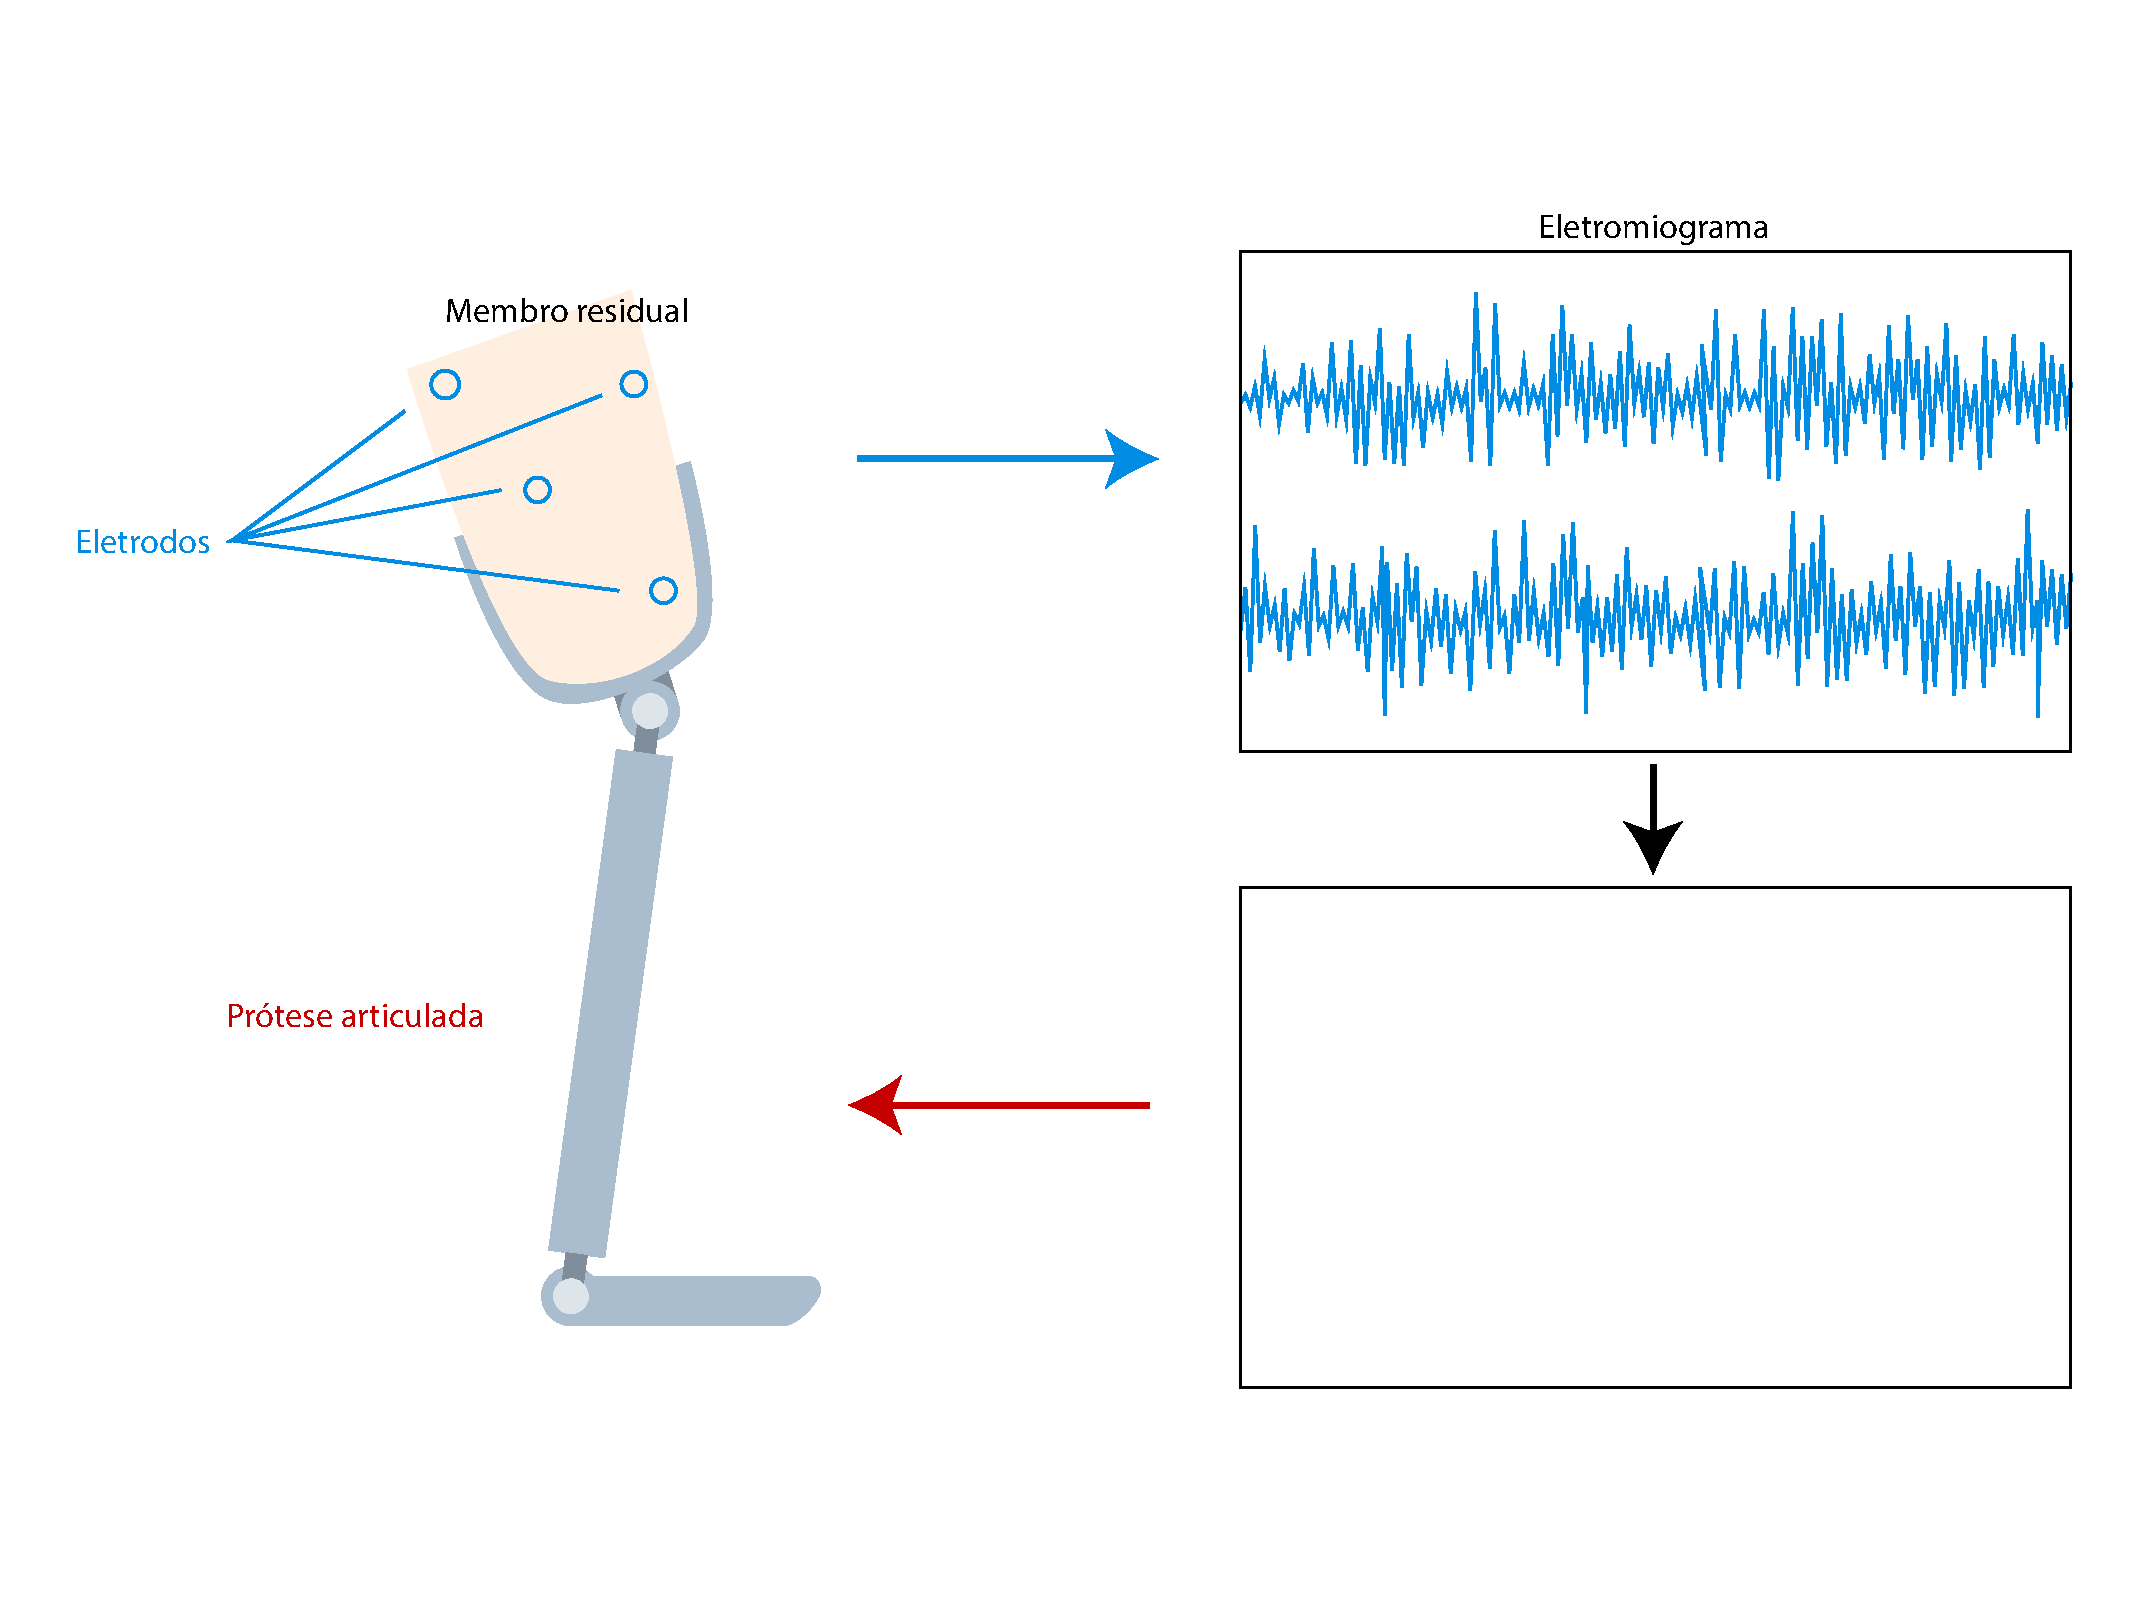
\includegraphics[width=0.7\textwidth]{resources/big_picture}}
	\end{center}
	\legend{Fonte: Elaborada pelo autor}
\end{figure}

O sistema computacional que envolve o projeto estará equipado com sensores flex nas articulações dos joelhos além de giroscópios e acelerômetros, que serão usados para capturar as ações do usuário. A \autoref{fig:big_picture} ilustra a visão geral do sistema, incluindo o posicionamento dos sensores e o atuador da prótese em si.

Os sensores serão posicionados nos joelhos do usuário, e os dados capturados serão transmitidos a uma placa de processamento, posicionada na estrutura da própria prótese, que fará a classificação para determinar a ação dos atuadores, como pode ser visto no fluxograma ilustrado na \autoref{fig:flowchart}.

\begin{figure}[ht]
	\caption{\label{fig:flowchart}Fluxograma de funcionamento da prótese}
	\begin{center}
	    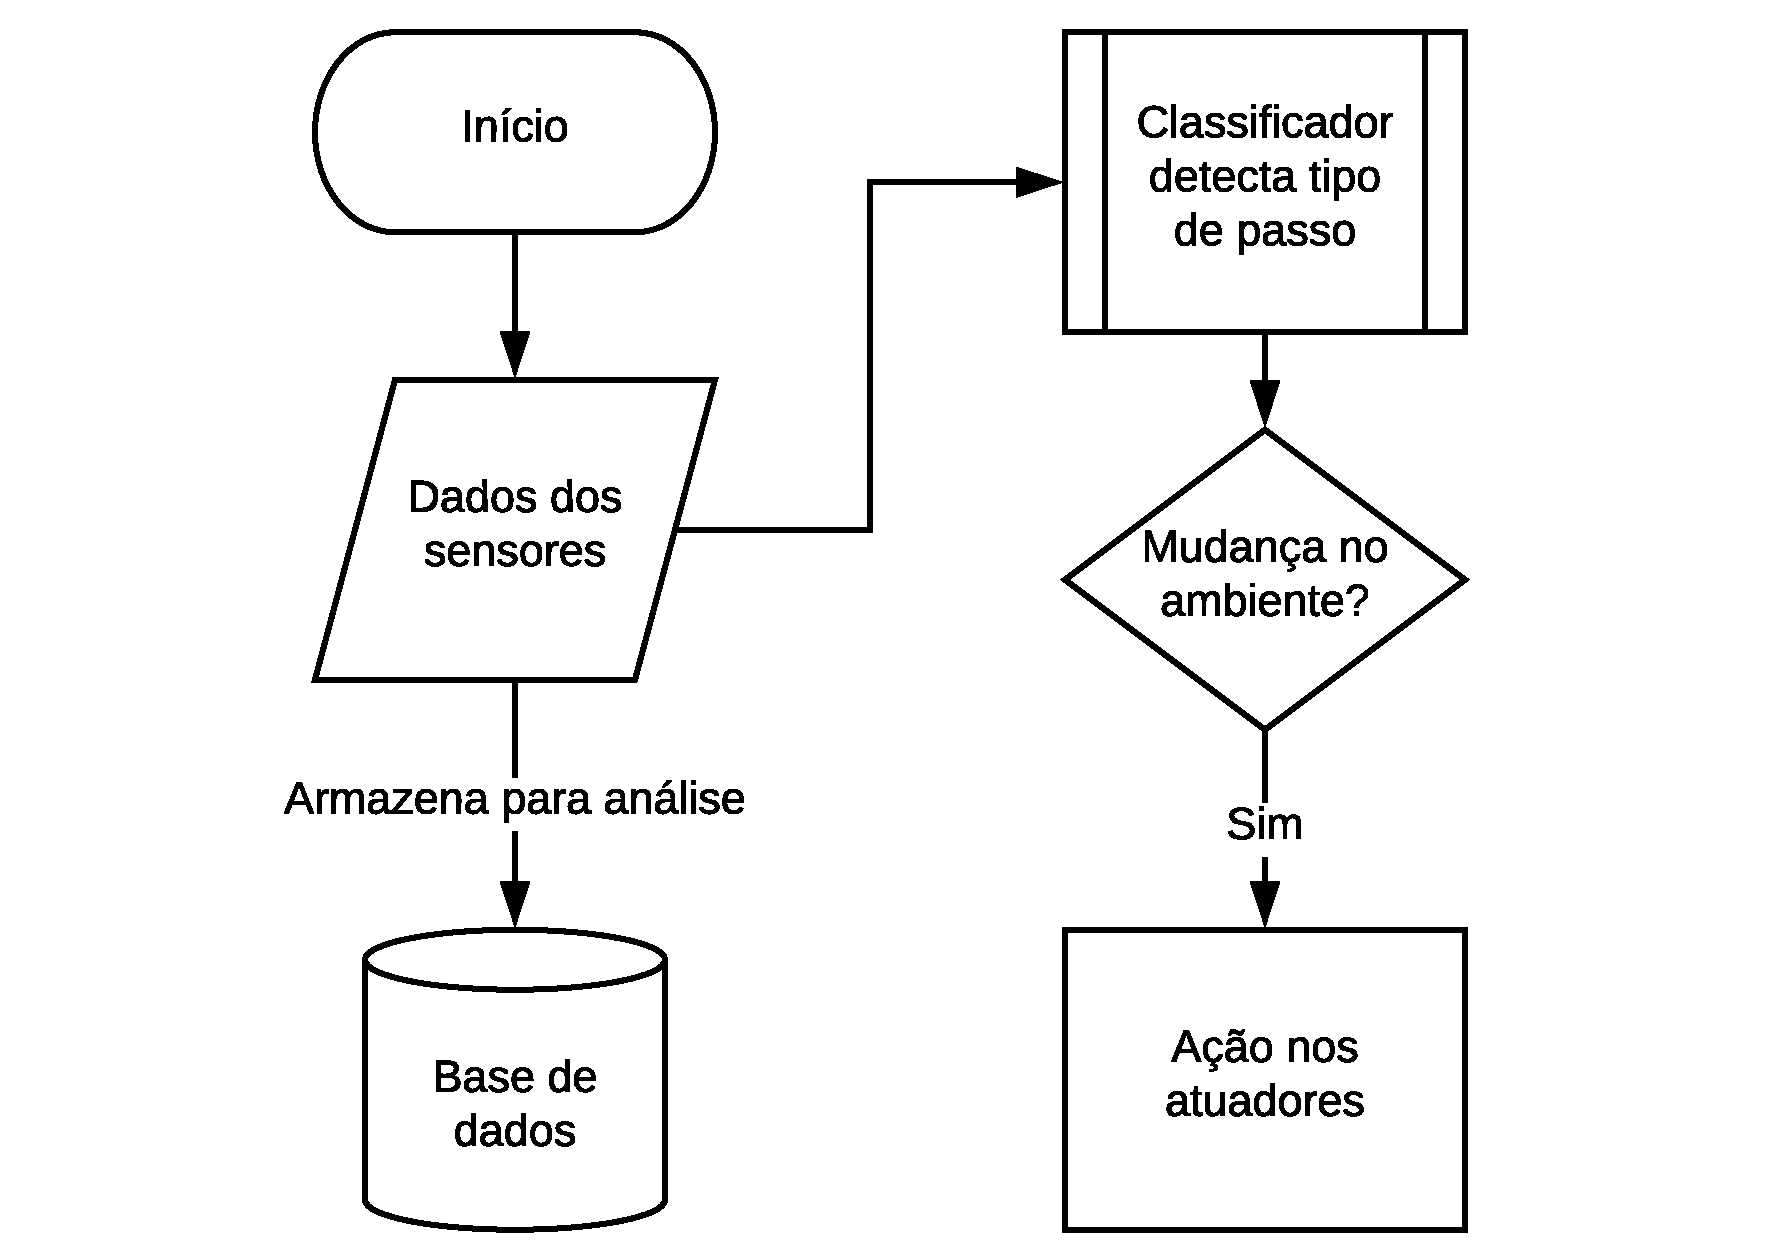
\includegraphics[width=0.8\textwidth]{resources/flowchart}
	\end{center}
	\legend{Fonte: Elaborada pelo autor}
\end{figure}


\section{Prototipação da prótese}\label{sec:metodo_prototipacao}
O diagrama de sequência da \autoref{fig:sequence_diagram} representa os componentes do sistema proposto por este trabalho, bem como a interação entre eles. Nela, pode-se observar a presença de dois objetos caracterizados como ``sensores'': com fio e sem fio. Os sensores sem fio são os localizados no membro intacto do usuário, que devem se transmitir os dados à central de processamento na prótese.

\begin{figure}[ht]
	\caption{\label{fig:sequence_diagram}Diagrama de sequência que descreve a interação entre os componentes do sistema}
	\begin{center}
	    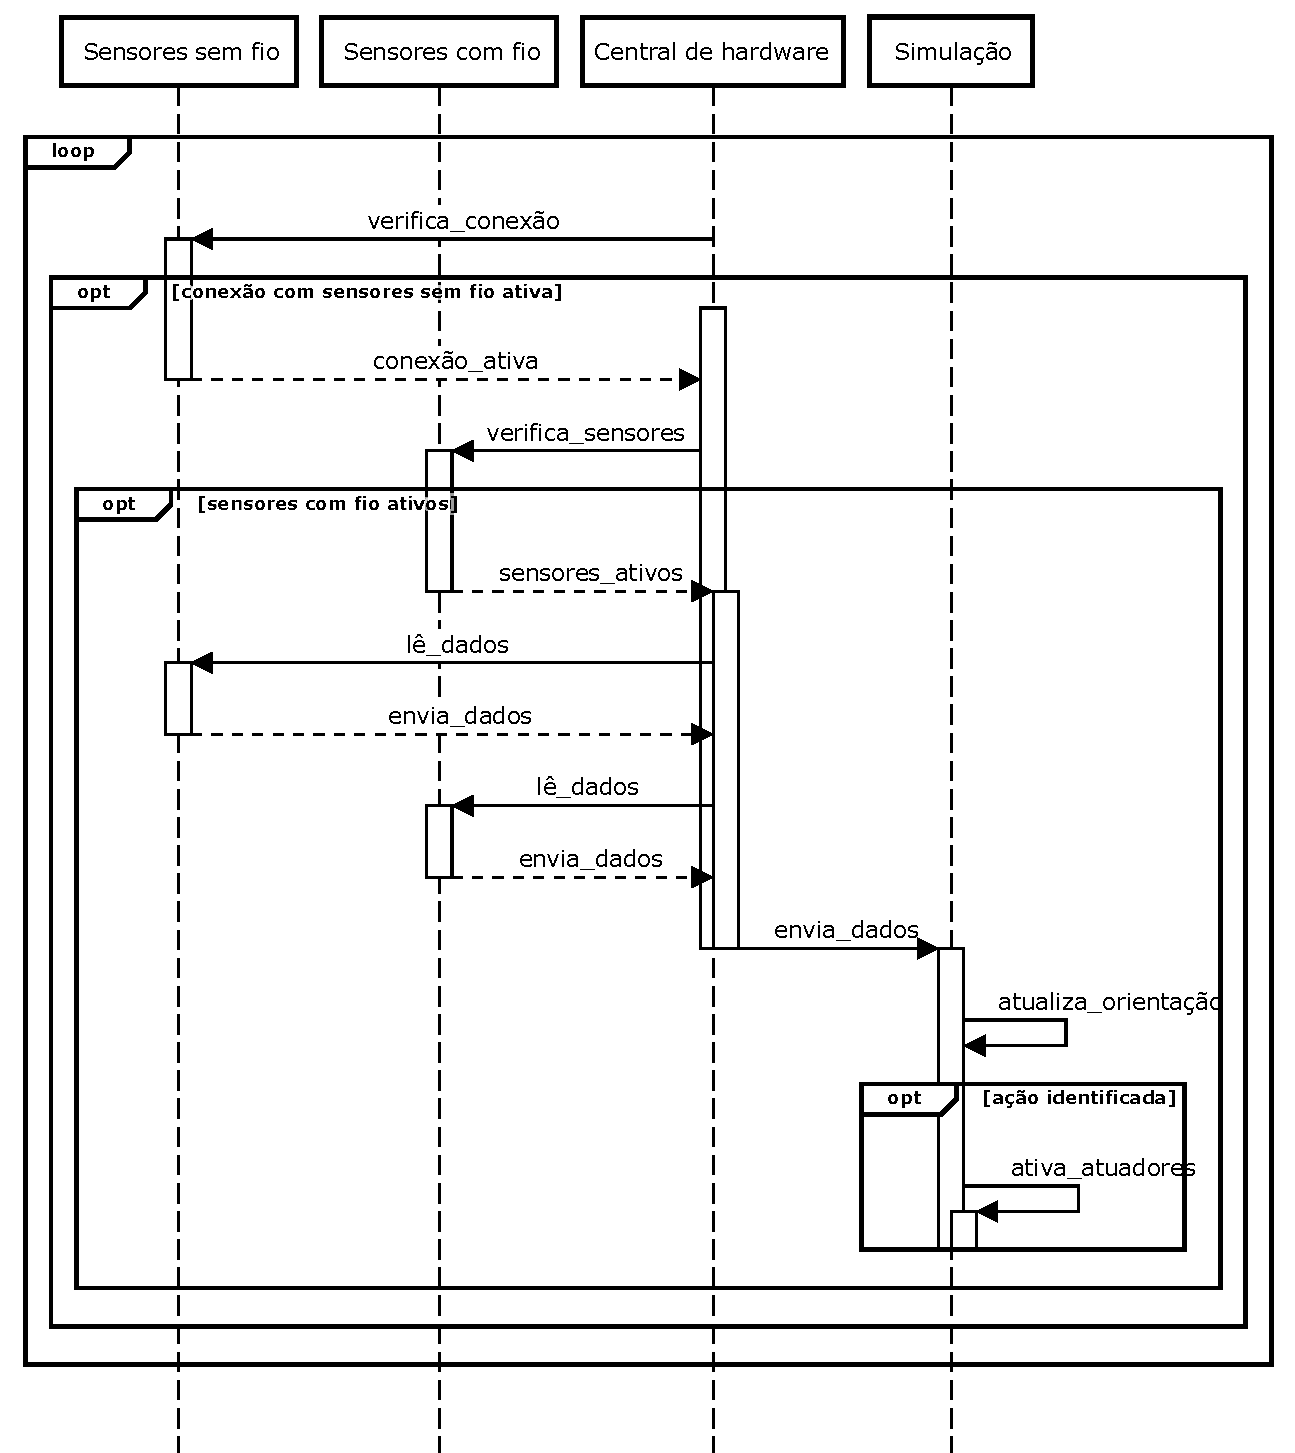
\includegraphics[width=\textwidth]{resources/sequence_diagram.pdf}
	\end{center}
	\legend{Fonte: Elaborada pelo autor}
\end{figure}

A central localizada na prótese deverá requisitar os dados dos sensores de forma constante, em um intervalo a ser determinado. Estes dados são então inseridos no classificador, que tomará a ação necessária e ativará os atuadores caso haja uma mudança de ambiente como, por exemplo, tenha sido iniciada a descida de uma escada.

\subsection{Arquitetura do software}\label{sec:metodo_prot_software}
% \todo[inline]{UML?}
\todo[inline]{Adicionar o que será apresentado nesta seção.}

\subsection{Arquitetura do hardware}\label{sec:metodo_prot_hardware}
A prótese em si será formada por partes impressas em 3D, feitas a partir de modelos gratuitos a serem escolhidos e adaptados. O uso de impressão 3D tem o intuito de manter o baixo custo do produto, que é um dos objetivos deste trabalho.

\begin{figure}[ht]
	\caption{\label{fig:hardware_scheme}Esquema representando o funcionamento dos atuadores}
	\begin{center}
	   \fbox{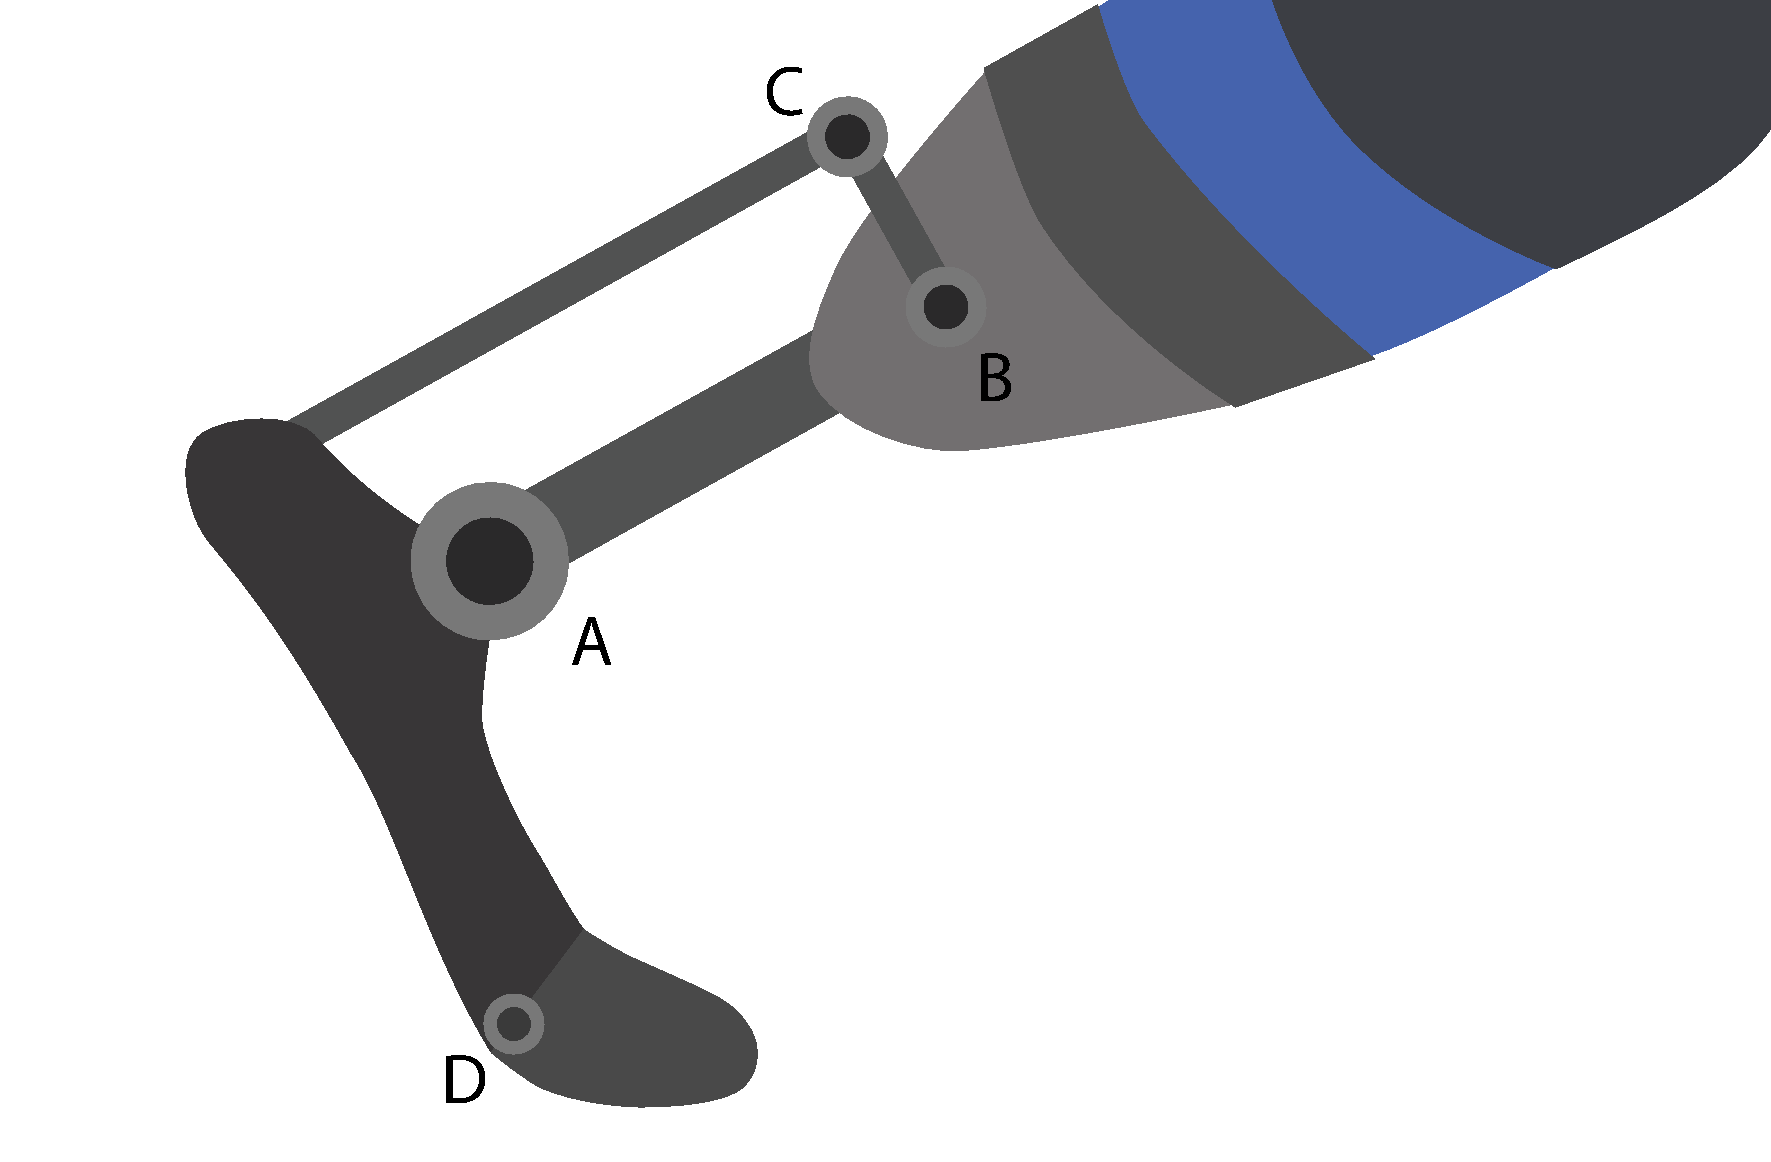
\includegraphics[width=0.5\textwidth]{resources/hardware_scheme}}	   %\missingfigure[figwidth=12cm,figheight=8cm]{Desenho de detalhe da prótese, com articulações, motores, etc.}
	\end{center}
	\legend{Fonte: Elaborada pelo autor}
\end{figure}

A~\autoref{fig:hardware_scheme} mostra o funcionamento dos atuadores do protótipo, que deverão ser acionados de acordo com a classificação dos dados dos sensores. No ponto A, o motor do ``tornozelo'' da prótese regulará a rigidez da articulação, como forma de manter estabilidade nos passos. Os pontos B e C referem-se a motores de passo que, juntos a hastes, se prendem no ``calcanhar'' da prótese, para mover o pé e exercer força na pisada.

Por fim, o ponto D da \autoref{fig:hardware_scheme} é uma articulação motorizada que manipula a parte dianteira do pé, afim de controlar a curvatura, simulando a flexibilidade de um pé humano. Alguns exemplos de configurações possíveis dos motores e articulações de acordo com diferentes cenários serão mostrados posteriormente na \autoref{fig:hardware_poses}.

\section{Coleta de dados}\label{sec:metodo_coleta}

Para que o sistema possa analisar e classificar os movimentos conforme o usuário utiliza a prótese normalmente, serão utilizados sensores nas duas pernas. Em cada joelho será posicionado um conjunto de um sensor flex, um giroscópio e um acelerômetro, que serão utilizados em conjunto.

Os valores capturados\todo{Adicionar um exemplo de dados gerados pelos sensores}\ pelos sensores do membro intacto serão transmitidos sem fios para a central de classificação dos sinais, que se conecta aos atuadores. Os sensores posicionados no membro residual se comunicarão diretamente através de fios com a central, pois estão posicionados fisicamente próximos. Os dados também serão armazenados para a análise descrita na~\autoref{sec:metodo_diagnostico}.

\section{Previsão de movimentos}\label{sec:metodo_previsao}
Os dados coletados serão analisados por um algoritmo de aprendizado de máquina para que se classifique e se preveja as ações do usuário. Essas ações serão classificadas de acordo com o passo a ser dado, podendo ser caminhada plana, subida ou descida de degrau.

Antes que o usuário realize um passo, o sistema deverá identificar em que ambiente este passo será dado. Isto poderá ser feito a partir do passo anterior, realizado pela perna intacta, e a partir do movimento atual extraído do membro residual.

Considerando que teremos um conjunto predeterminado de cenários possíveis -- caminhada plana, subida e descida de escada -- será decidida uma técnica de aprendizado de máquina supervisionado, mais especificamente de classificação, através de ferramentas de aprendizado de máquina, como as descritas na Seção~\ref{sec:ml_tools}.

\begin{figure}[h]
	\caption{\label{fig:hardware_poses}Algumas posições da prótese de acordo com cenários}
	\begin{center}
	   \fbox{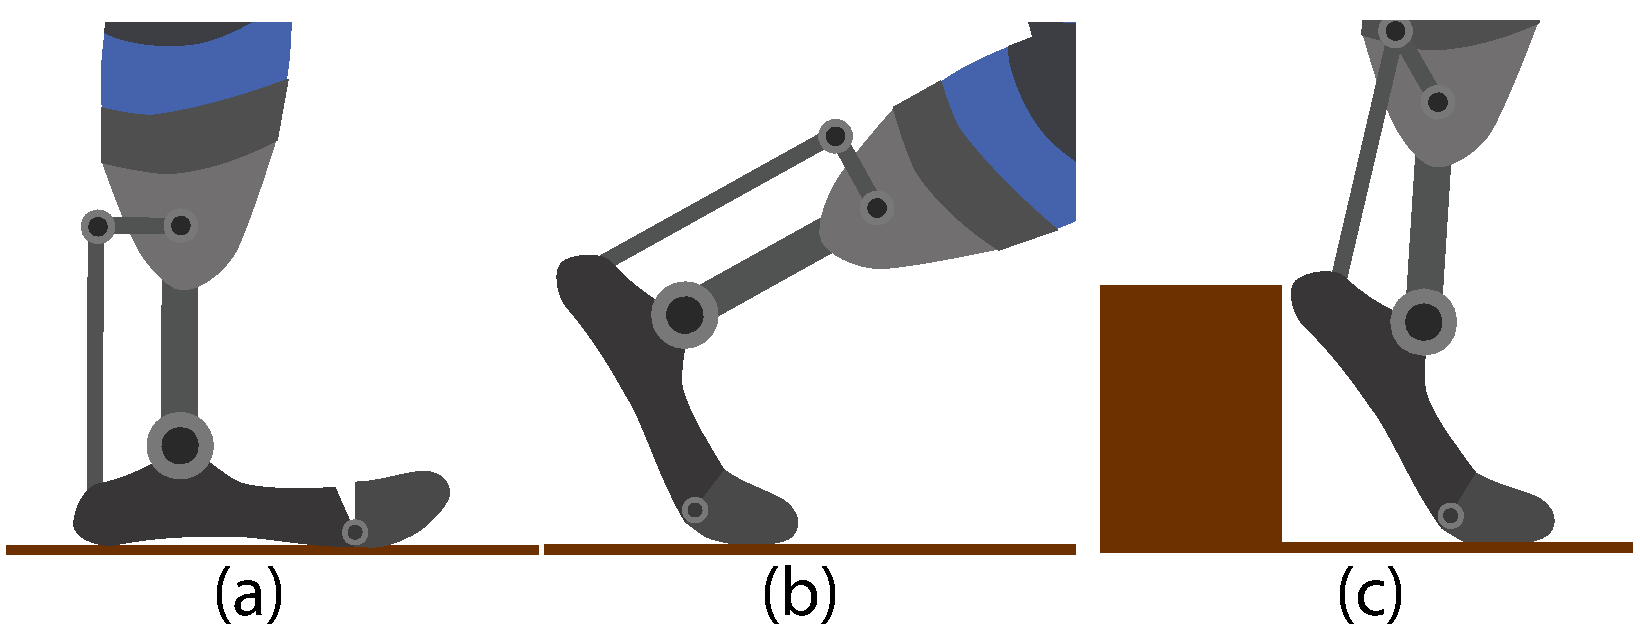
\includegraphics[width=\textwidth]{resources/hardware_poses}}
	   %\missingfigure[figwidth=12cm,figheight=5cm]{Poses da prótese em diferentes situações: início de caminhada, fim de caminhada, descida de escada.}
	\end{center}
	\legend{Fonte: Elaborada pelo autor}
\end{figure}

Assim que um passo começa a ser realizado, classifica-se o tipo de passo a ser realizado, e acionam-se os atuadores, que terão sua ação determinada de acordo com o cenário identificado. Na~\autoref{fig:hardware_poses} pode-se observar a forma em que a prótese deve se posicionar de acordo com cada tipo de ação. As ações diferem para o início e o fim de cada passo em diferentes cenários.

As três ações representadas na \autoref{fig:hardware_poses} referem-se a (a) pisada plana, (b) fim de um passo em piso plano, e (c) descida de escada. No primeiro caso, os motores só mantém estabilidade para garantir equilíbrio; no segundo caso, é necessária maleabilidade na dianteira do pé, para que seja possível impulsionar o passo do usuário. No terceiro caso, antes que o usuário desça o próximo degrau, a prótese deve inclinar-se e contrair a dianteira do pé para evitar tropeços e auxiliar na descida.

\section{Diagnóstico do uso da prótese e recomendações de melhorias no caminhar}\label{sec:metodo_diagnostico}
Os dados dos sensores também serão automaticamente armazenados para geração de estatísticas que podem ser usadas para diagnóstico relacionado à saúde da caminhada do usuário. O sistema fará um relatório do uso, indicando se é exercida mais força em uma das pernas do que na outra, por exemplo, além de outros dados.

A partir das informações geradas, poderá ser feitas recomendações de melhorias ao indivíduo, para que se melhore a postura, a caminhada, ou que se utilize algum tipo de equipamento adicional. Além disso, ainda será possível analisar as estatísticas de uso da prótese para avaliar seu impacto na vida do usuário, caso esteja alterando seus hábitos de alguma forma.

Para que este diagnóstico seja possível, será analisada a hipótese do uso de sensores adicionais aos propostos pelo protótipo atual, caso estes não sejam suficientes para gerar os dados necessários de análise de saúde da caminhada.